\chapter{Background and Introduction}
\label{chIntro}

\section{Diamond in Quantum Technology}
\indent
	
	Aside from diamond's status in the jewelry industry, the physical properties of diamond have driven its popularity in a wide range of applications. Diamond is mechanically hard, resistant to chemical corrosion, biologically compatible, an ultra wide-bandgap semiconductor \cite{PaulM2000}, and has high carrier mobilities \cite{Isberg2002} making it suitable for polishing hard materials like stainless steel \cite{Ranjan2019}, targeted drug delivery \cite{Man2012}, high power electronic devices such as Schottky diodes \cite{Nicley2015}, and quantum technologies \cite{Greentree2008}. Quantum applications of diamond cover a wide range from magnetic field sensing \cite{Maze2008} to communications \cite{Lin2019} and quantum computing \cite{Weber2010} making diamond materials research a field of high impact.

	Diamond is particularly suitable for quantum applications for several reasons. First, as an ultra wide bandgap semiconductor with a bandgap approximately five times larger than silicon's, diamond has the ability to host a number of different defects without the electronic structures of those defects interfering with the electronic structure of the diamond host material \cite{Weber2010}. Second, carbon-12 has a relative abundance of 98.89 \% and carbon-12 isotope enriched samples and sources can be used to further improve the purity. Carbon-12 has zero nuclear spin which is important for quantum applications as nuclear spins near a quantum defect are a source of decoherence. These two properties allow the defects in diamond to exist as isolated atoms in what is essentially, a spin-free bath.
	
	Diamond defects are also called color centers because the electronic structure of the defects transmit and absorb visible light giving color to otherwise transparent host diamond. A few common color centers include: nitrogen vacancy defect (NV), silicon vacancy defect (SiV), tin vacancy defect (SnV), and the nickel vacancy defect (NiV). Slight differences in defects make them more or less suitable for different applications. While the others are better suited for quantum communication and quantum computing, the nitrogen vacancy center appears best suited for quantum sensing applications \cite{Achard2020}. The NV defect is not ideal for quantum communication and computing applications because it has poor optical properties that result from weak zero phonon line (ZPL) emission and a large phonon side band. Alternatively,  NV defects have long spin coherence times because they are a spin-1 system which means they do not couple to the spin-1/2 bath in the host material. Long coherence times are crucial for quantum sensing applications.
	
%	Weber \textit{et al.} identified several important criteria for a defect and host system that make for successful quantum computing \cite{Weber2010}. The criteria for the host material include: a wide bandgap to prevent interference with the optical transition of the defect, small spin-orbit coupling, availability as high quality bulk or thin film single crystal, made up of elements that have zero nuclear spin in their naturally occurring isotopes \cite{Man2012}. Diamond fits the criteria for an ideal host material for quantum computing because of its wide bandgap, the abundant isotope of carbon-12 having zero nuclear spin, a small spin-orbit coupling, and the advancements in synthetic diamond growth that yield high quality single crystal diamond (SCD). The defect criteria include: a bound state fitting for a qubit, an optical pumping cycle that polarizes the qubit state, differentiable luminesce in qubit sublevel states, optical transitions that do not interfere with the host material electron states, and separation in bound states that are large enough to not transition due to thermal excitation \cite{Weber2010}. Diamond has a broad range of defects, also termed color centers, due to point defects acting as isolated atoms and the wide bandgap allowing the defect to transition without affecting the electronic states of the diamond itself \cite{PaulM2000},\cite{Weber2010}. One of the most common color centers in diamond is the negatively charged nitrogen vacancy center (NV-). Evidently, the NV- in diamond fits the criteria laid out by Weber \textit{et al.} which is why it has become a front runner in quantum technology research \cite{Weber2010}. 

\section{The Nitrogen Vacancy Defect as a Quantum Sensor}
\label{NVintro}
\indent
	
	The negatively charged nitrogen vacancy defect (NV$^{-}$) is comprised of a single substitutional nitrogen on a carbon lattice site with a vacancy on an adjacent lattice site. The negative indicates the defect has trapped an additional electron \cite{GDavies1976}. The energy diagram for the NV$^{-}$ defect is shown in Figure \ref{fig: NVEnergyLevels} \cite{Mzyk2022}. There are several important properties of the NV$^{-}$ center that make it well suited for quantum sensing applications \cite{Weber2010}. First, the quantum state can be polarized via optical pumping. In Figure \ref{fig: NVEnergyLevels}, the metastable intersystem crossing polarizes the state to the m$_s$=0 state because there is a strong spin-orbit coupling with the excited m$_s$=$\pm$1 state and the intersystem crossing but a weak spin-orbit coupling with the excited m$_s$=0 state and the intersystem crossing. Over time, this results in a higher probability that electrons will be in the m$_s$=0 state. Because of the quantum state polarization resulting in higher probabilities that electrons will be in the m$_s$=0 state, the m$_s$=0 state presents brighter than the state m$_s$=$\pm$1 giving a luminescent distinction between states. Lastly, Figure \ref{fig: NVEnergyLevels} shows the Zeeman Effect in the NV$^-$ center. When a magnetic field is applied, the separation between the m$_s$=+1 and m$_s$=-1 dark states increases proportionally to the strength of the field. This property of the NV$^-$ center is one way it can be used to sense magnetic fields. NV$^-$ centers can also detect magnetic fields through phase accumulation. Here, the state of the NV$^-$ defect is projected onto the x-y plane of the Bloch sphere where it evolves in time until the state is read out. The long coherence times of NV$^-$ defects allows the phase information to be preserved while in the x-y plane of the Bloch sphere.
	
	%possibly  mention temperature splitting and how this can be used for temperature sensing if more content needed
    \begin{figure} [ht]
        \centering
        \includegraphics[scale=0.4]{figures/NVEnergyLevels_Mzyk2022.png}
        \caption{Energy level diagram for the NV$^{-}$ defect as shown above \cite{Mzyk2022}}.
		\label{fig: NVEnergyLevels}
    \end{figure}
	
	    
    To more broadly utilize the nitrogen vacancy defect for quantum sensing applications, controllable and repeatable manufacturing of NV$^-$ centers in high-quality SCD is necessary. Repeatable and controllable manufacturing means the type, quantity, and location of the NV$^-$ centers must be consistent with respect to processing parameters, e.g. if a sample is grown using Process A, the nitrogen will incorporate as substitutional nitrogen at a quantity of 5 ppm in the 10 nm layer in the vertical center of the grown crystal.

    \textcolor{red}{** I think I need to talk more about the array of NVs for improved spatial resolution and why the NVs need to be in a subsurface layer**}
    
	%	The NV\unit{^{-}} center in diamond exhibits quantum spin properties with three unique spin states: up, down, or mixed \cite{Savage2021}. These spin properties and the ability to manipulate the spin state makes the NV\unit{^{-}} center a strong candidate for a quantum sensing.  The NV\unit{^{-}} center has two triplet states, ground and excited, and an intermediate singlet state \cite{Mzyk2022}. 
	%	The spin state of an NV- center can be manipulated using a combination of visible light and microwaves. To promote electrons of either spin from the ground state to the excited state, a diamond sample with NV- defects can be illuminated with a green laser, 533 nm, which provides the electrons enough energy to occupy the excited band in the energy structure for the NV- defect \cite{Mzyk2022} without giving it enough energy to promote the electron to the conduction band of the diamond, again, due to its wide bandgap, thus fulfilling the first criterion of the ideal quantum host material and the fourth criterion of the ideal quantum defect as identified by Weber \textit{et al.} \cite{Weber2010}. Because the excited state is not stable, the electron relaxes to the ground state of the same spin by releasing a photon of red light. A non-radiative transition through the intermediate singlet can also occur in which case a phonon is released. The non-radiative transition through the intermediate singlet favors the m¬¬s=0 ground state, which is how the second defect criteria, optical pumping that polarizes the qubit state, identified by Weber \textit{et al.} is achieved \cite{Weber2010}, \cite{Mzyk2022}. The spin states manipulation results in a drop in fluorescence when sweeping through microwave frequencies in an optical detected magnetic resonance (ODMR) measurement \cite{Mzyk2022}. The microwave frequency where the drop in intensity occurs indicates the energy needed to change the spin from ms=0 to ms=±1 \cite{Mzyk2022}. The difference in intensity satisfies Weber \textit{et al.} third ideal quantum defect criterion \cite{Weber2010}. Research on creation of NV- in a specific orientation by utilizing step flow CVD growth and substrates of favorable orientation \cite{Lesik2015}, improving coherence times, and devices with NV- qubit system, which requires spatial control in the formation of the NV- center continues.
	
	%discuss PL, overview, uses, results, etc.

\subsection{Nitrogen Vacancy Defect}
\subsubsection{Step 1: Synthetic Diamond}
\label{syntheicDiamond}
\indent
    
    The first step to repeatable and controllable manufacturing of NV$^-$ defects is repeatable manufacturing of diamond. Diamond is an allotrope of carbon that is not thermodynamically favorable at standard temperature and pressure; under these conditions, the thermodynamically favorable allotrope is graphite \cite{PaulM2000}. Diamond is naturally produced in the Earth’s mantle, because the mantle provides the high pressure high temperature environment necessary to achieve thermodynamic stability. Diamond then travels to the surface where it can be mined for jewelry, for example. Diamond can also be synthetically grown using high pressure high temperature (HPHT) techniques or chemical vapor deposition (CVD). Synthetic diamond properties can be more repeatable than natural diamonds because of the control over growth conditions and ability to monitor key reaction parameters. 

    \noindent\textbf{High Pressure High Temperature (HPHT) Diamond}
    \newline\indent
     The HPHT technique achieve thermodynamically favorable conditions for the diamond allotrope of carbon. Here, a carbon containing material, such as graphite, is combined with molten metal in a reactor under high pressure, high temperature conditions matching those in the Earth’s mantle \cite{Bovenkerk1993}. After several days to months, the reactor is then decompressed and the diamond sample is removed. This technique can produce large single crystal diamonds, several millimeters in size \cite{Sumiya1996}. However, this technique does not allow \textit{in situ} control of reactor parameters.

    \noindent\textbf{Chemical Vapor Deposition (CVD)}
    \newline\indent
    The second technique to synthetically produce diamond is CVD. This technique exploits the kinetics aspect of the reaction by focusing on adding one gaseous carbon radical at a time to an existing seed crystal to grow the SCD \cite{PaulM2000}. The seed crystal can be diamond (homoepitaxy) or a different crystal(heteroepitaxy). Homoepitaxal growth results in less strain in the grown film. To minimize the strain introduced into heteroepitaxial grown films, the seed crystal should have a similar lattice parameter and crystal structure. In this technique, a gaseous \textit{sp$^3$} hybridized carbon in a predominately hydrogen gas phase attaches to the dangling \textit{sp$^3$} hybridized carbon atom in the diamond lattice at the surface of the seed crystal \cite{PaulM2000}. It is crucial to have a predominately hydrogen gas phase because hydrogen favorably etches graphitic carbon, \textit{sp$^2$} hybridization, thus leaving the hybridized carbons that favor the diamond lattice  \cite{PaulM2000}. Figure \ref{fig: CVDSchematic} provides a graphical representation of the \textit{sp$^3$} hybridized carbon radicals attaching to the dangling bonds that were exposed by hydrogen radical. This technique yields a sort of layer-by-layer approach as opposed to the bulk transition to SCD that occurs in the HPHT technique.

    The more incremental approach to diamond growth via CVD, as opposed to the more bulk process of HPHT grown SCD, facilitates \textit{in situ} process changes to control the final product. For example, the gas phase composition could be altered for some amount of time and then returned to its initial composition resulting in a layered structure. This was demonstrated by Lobaev \textit{et al.} for nitrogen in a laminar flow reactor \cite{Lobaev2017}. For this reason, chemical vapor deposition is a promising technique for spatial control of the nitrogen incorporated in growing single crystal diamond; a crucial aspect of repeatable and controllable manufacturing of NV centers in diamond. Chemical vapor deposition of synthetic diamond will be discussed in more detail in chapter \ref{DiamondGrowth}.
	
       \begin{figure}[ht]
           \centering
       	\includegraphics[scale=0.6]{figures/CVDSchematic_May2000.png}
        	\caption{Creation of \textit{sp$^3$} dangling bonds at the seed surface that provide a bonding site for \textit{sp$^3$} carbon radicals in the gas phase \cite{PaulM2000}.}
      	\label{fig: CVDSchematic}	
       \end{figure}
% CVD reactors exist in many different designs including hot filament or microwave plasma assisted designs which differ in their method for carbon radical production \cite{PaulM2000} and two different geometries for CVD reactors include bell jar and tube flow reactors where each design fills a certain niche for the CVD process \cite{Dahmen2003}. For example, microwave plasma assisted CVD (MPACVD) reactors have an advantage over the hot filament CVD reactor design, even though the hot filament design operates at a lower cost, because, in the MPACVD reactor, a bias can be applied to the substrate to stimulate faster growth rates because the plasma density near the substrate can be increased \cite{PaulM2000}. Similarly, the different geometries offer unique benefits. The tube flow reactors offer faster resonant times \cite{Lobaev2017}, thus faster switching of the gas phase composition which can lead to higher precision \textit{in situ} delta doping, whereas the bell jar reactor offers a larger surface where deposition on several substrates can occur at the same time because of the overall size of the reactor and the ability to adjust the electromagnetic modes in the chamber to promote wide, flat plasmas across all the samples \cite{Bovenkerk1993}, \cite{Lobaev2017}. Research in improving quality, growth rate, and overall size of single crystal diamond is being pursued. 

\subsubsection{Step 2: Nitrogen Incorporation in Diamond Lattice}
\indent
    The necessary steps to fabricate NV$^-$ defects are nitrogen incorporation, vacancy formation, and NV center creation. Nitrogen can be incorporated post process via ion implantation or \textit{in situ} during synthetic diamond growth. 


\noindent\textbf{Ion Implantation}
 \newline\indent 
 For ion implantation to fabricate NV$^-$ defects, nitrogen ion are accelerated towards a diamond substrate where they bombard the surface at a set fluence (electrons/cm$^2$). The high energy nitrogen atoms enter the diamond substrate and knock carbon atoms off lattice sites, creating some vacancies, or fill interstitial sites. The depth nitrogen ions penetrate into the diamond substrate is dependent on the accelerating voltage whereas the quantity of nitrogen is dependent on fluence and time of implantation. This technique introduces lattice damage and inhomogeneous strain.

\noindent\textbf{\textit{In situ} Doping}
    \newline \indent
    An alternative is \textit{in situ} CVD doping. Here, nitrogen is introduced into the gas phase of the CVD reactor. The nitrogen can then incorporate at the \textit{sp$^3$} dangling bonds, as shown in Figure \ref{fig: CVDSchematic}, creating single substitutional nitrogen defects (P1 centers). Depth control of single substitutional nitrogen using \textit{in situ} doping in CVD can be done by introducing and removing the nitrogen in the gas phase at set times.
	

\subsubsection{Step 3: Vacancy Formation in Diamond Lattice Diamond}
\indent
	The next step in creating NV$^-$ defects is to form vacancies. Vacancies can be introduces through irradiation processes. Irradiation is similar to ion implantation in that the sample is bombarded. However, irradiation does not have to be done using ions; it can be ultraviolet irradiation \cite{GDavies1976} or electron beam irradiation \cite{Luo2021}, for example. If ion implantation was used to incorporate nitrogen, some vacancies form during the ion implantation process. For \textit{in situ} CVD doping, additional vacancies can be formed with electron beam irradiation. Again, accelerating voltage, fluence, and irradiation time determine depth and concentration of vacancies. 
    
\noindent\textbf{Electron Beam Irradiation}
\newline \indent
	One example of electron irradiation and annealing being used to form NV defects was completed by Luo \textit{et al.} \cite{Luo2021}. Here, four CVD substrates were electron irradiated and annealed. The absorption spectra of the four samples were characterized after each step and compared. Figures \ref{fig: AbsAfterIrr} and \ref{fig: AbsAfterIrrAndAnneal} show absorption spectra of four samples irradiated at the same electron energy but different fluence pre- and post- annealing, respectively \cite{Luo2021}. All four samples were CVD grown under the same conditions from CVD seeds that were laser cut and removed to prevent contribution to the spectra from the seed \cite{Luo2021}. A spectrum of the as-grown sample was used as a background and subtracted from each spectrum to show the change in defect due to the irradiation or annealing process. The peak at approximately 393 nm is a result of the negatively charged vacancy, V$^-$, defect \cite{Luo2021}. The intensity of the peak is proportional to the concentration of the defect. Therefore, Figure \ref{fig: AbsAfterIrr} demonstrates an increase in V$^-$ concentrations as the fluence increases \cite{Luo2021}. Additionally, the peak at approximately 741 nm within a broad side band from approximately 500-750 nm, which is attributed to the neutral vacancy defect (V$^0$), in Figure \ref{fig: AbsAfterIrr} increases with increasing fluence \cite{Luo2021}. Both observations are logical because increasing fluence means more electrons per unit area are hitting the sample and knocking atoms off lattice sites. Because these samples are being irradiated with an electron beam, it is also logical that the V$^-$ occurs at higher concentration than the V$^0$ because the increase in number of electrons bombarding the sample introduces more electrons into the sample for a vacancy to potentially trap. 

\section{Laser Writing}
	Finally, the incorporated nitrogen and vacancies must come together to form NV defects. The annealing process promotes diffusion of the nitrogen and vacancy species. It is known that vacancies tend to settle adjacent to single substitutional nitrogen centers \cite{Savage2021}. Additionally, the annealing process reduces the free energy of the system. This is crucial because the implantation and irradiation processes introduce damage to the diamond lattice and inhomogeneous strain both of which are detrimental to the operation of the NV$^-$ defect in quantum sensing applications.
	

	
	%Ion implantation and electron beam irradiation introduce nitrogen as both interstitials and single substitutional nitrogen (P1 centers) as well as electron and vacancies. These processes do not necessary produce NV$^-$ centers. 
	
	%to a location adjacent to P1 center include irradiation and annealing.  Electron beam (e-beam) irradiation is commonly used for creation of vacancies. The electrons bombard the sample with some fluence (electron/cm$^2$) and accelerating voltage and knock atoms off of lattice sites thus creating vacancies \cite{Savage2021}. Time of irradiation, accelerating voltage, and fluence can be optimized to achieve the chosen vacancy concentration and depth. After irradiation, annealing is performed to promote movement of the vacancies, and it is known that many vacancies settle adjacent to substitutional nitrogen \cite{Savage2021}. 
	
	\begin{figure}[ht]
        \centering
		\includegraphics[scale=0.5]{figures/AbsAFterIrr.png}
		\caption{Absorption spectra of 1MeV irradiated samples, prior to annealing, of varying fluence. The as-grown absorption spectrum has been subtracted from each data set \cite{Luo2021}.}
		\label{fig: AbsAfterIrr}
	\end{figure}

	\begin{figure}[ht]
        \centering
		\includegraphics[scale=0.5]{figures/AbsAFterIrrAndAnneal.png}
		\caption{Absorption spectra of 1MeV irradiated sample of varying fluence and annealed. The as-grown absorption spectrum has been subtracted from each data set \cite{Luo2021}.}
		\label{fig: AbsAfterIrrAndAnneal}
	\end{figure}

	Figure \ref{fig: AbsAfterIrrAndAnneal} shows the same four samples after annealing \cite{Luo2021}. The NV$^-$ peak occurs at 637 nm and is accompanied by a broad phonon side band extending to ~450nm \cite{Luo2021}; in both spectroscopic features, intensity increases as the fluence increases. The NV$^0$ peak occurs at 575 nm, within the broad phonon side band of the NV$^-$. However, the NV$^0$ peak becomes visible for the sample with 1$\times$10$^{18}$ e/cm$^2$ and 3$\times$10$^{18}$ e/cm$^2$ fluence \cite{Luo2021}. Figure \ref{fig: AbsAfterIrrAndAnneal} also indicates an excess of vacancies that did not form NV$^{-/0}$ centers because the 741 nm and 393 nm peaks are still visible, more notably at high fluence \cite{Luo2021}. High fluence is expected to produce more vacancies due to the higher flux of the electrons and vacancies do not always find a P1 defect during annealing. In any case, the concentration of NV$^-$ defects within the samples increased through the irradiation and annealing processes. The shortcoming of this process is, again, the lack of spatial control of the NV$^-$ center formation. 
	
	Recently, Chen \textit{et al.} demonstrated a localized irradiation and annealing process with \textit{in situ} characterization to create isolated single NV$^-$ defects \cite{Chen2019}. Here, an HPHT diamond with approximately 1.8 ppm of single substitutional nitrogen defects was irradiated with a laser pulse to create an ensemble of vacancies, in a region where no NV centers were previously observed, followed by irradiation with lower energy pulses to locally anneal \cite{Chen2019}. During the “annealing pulses,” the fluorescence of the region was monitored so that once an NV$^-$ center was detected, the pulses stopped, thus creating a single NV$^-$ center \cite{Chen2019}. 
	

\subsection{Current Limitations}
    The laser writing technique can place nitrogen vacancy defects within approximately 40 nm in XY spatial resolution \cite{Chen2019}. In Z spatial resolution, however, is approximately 200 nm \cite{Chen2019}. The significant variation in depth of nitrogen vacancy centers affects the coherence time and signal strength. Further improvements in depth control of nitrogen vacancy center placement is necessary to further improve quantum sensing with NV$^1$ centers.
    
\subsection{Characteristics of an Ideal Substrate}
    One potential solution to improving depth control of nitrogen vacancy centers using laser writing is to control the position of the nitrogen within the substrate. Introducing a single crystal diamond seed with controlled nitrogen concentration in a delta doped layer as opposed to the HPHT seed would allow for improved spatial control of the NV$^-$ defect.
    
    \begin{figure}[h!]
    \centering
    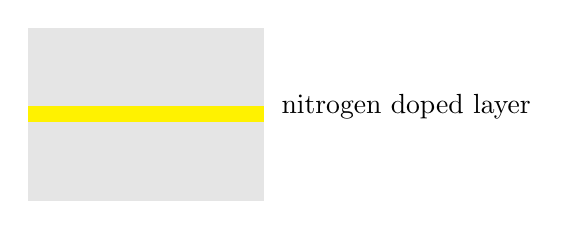
\begin{tikzpicture}
        % Bottom gray box
        \fill[gray!20] (0,0) rectangle (3,1);
    
        % Thin yellow box in the middle
        \fill[yellow] (0,1) rectangle (3,1.2);
        \node[anchor=west] at (3 + 0.1, 1.2) {nitrogen doped layer};

        % Top gray box
        \fill[gray!20] (0,1.2) rectangle (3,2.2);
    \end{tikzpicture}
    \caption{Visual representation of delta doped layer.}
    \end{figure}

	